\section{Introduction}
\label{sec:intro}
Since stone age, humans use fuels, defined as any energy carriers intended for energy conversion \cite{FAO_biofuel, ISO16559}. First evidence of the use of domesticated fire was established in 790 000 B.C. \cite{alperson2010acheulian}. Thus, biomass has been the first fuel used by the human kind for security, cooking and heating. Nowadays, most of the used energy sources are fossil fuels. In 2019, oil, coal and gas represented respectively 31\%, 25\% and 23\% of the global primary energy consumption \cite{ourworld_2019}. Despite their great advantage, high energy density, these fuels have a major drawback: their combustion releases huge quantities of carbon dioxide (35 Gt of \ce{CO2} in 2019) mainly responsible for climate change \cite{iea2020world}. The biggest challenge of the energy transition is to secure the energy supply while reducing the greenhouse gas emissions. In practice, this means finding alternatives to fossil fuels.

First and foremost, in the context of the energy transition, fuels will keep playing a major role in the global energy system \cite{Ahlgren2012}. Even if electricity gains shares through the electrification of the energy demand, it will not entirely displace fuels for three main reasons: storage, infrastructure compatibility and cross-sectorial links. Because of their intermittency and space disparity, a deeper integration of \gls{VRES} requires storage and transport in order to supply the energy demand at the right time and in the right place \cite{Brouwer2016,Evans2012,Gallo2016,hall2008,Rosa2017}. Where typical container of batteries are limited in terms of storage capacity (up to 10~MWh) and present significant costs and self-discharge losses, the energy conversion into fuels provides a more affordable solution for higher storage capacity (from 100~GWh) and longer storage time scales (months to year) \cite{Rosa2017}. Due to the economic inertia and their infrastructure legacy \cite{Ahlgren2012}, fuels remain the most appropriate solution for sectors requiring high energy density (\eg heavy-duty transport, shipping, aviation or chemical industry) \cite{Albrecht2020,Decker2019,Goede2018,Pearson2012,Rosa2017,Stancin2020,Trieb2018,Zeman2008}. 
\citet{contino2020whole} point out that the energy transition is an interdisciplinary effort and not solely about the power sector. The latter represents only a fifth of the global energy consumption \cite{iea_renewable}. Also, \citet{Goede2018} has shown in 2018 that \ce{CO2} emissions of the Netherlands are equally apportioned between the different types of end-use-demands (\ie power, heat, mobility and non-energy). This highlights the necessity to consider every energy sector rather than focusing all efforts on the power system and even more, to shift towards a multi-vector interconnected energy system. In this cross-sectorial approach and with the perspective of increasing shares of \gls{VRES}, fuels are promising energy carriers in order to maximise the overall system efficiency \cite{mathiesen2015, Stancin2020}.

Given the growing diversity of pathways for transforming the renewable energy sources into fuels, clear classification and terminology are necessary \cite{bailera2017}. As predicted by \citet{ridjan2016}, there is now a need to support the right fuel technology development, via the use of a more comprehensive and quantitative terminology (\eg specifying the share of biomass in the energy balance of the production of a biofuel). The objective of this terminology is to avoid the confusion between these fuels and thereby reduce misunderstanding in political or academic discussions. To a further extent, such an harmonisation may help ``to facilitate comparison between national fuel market and enhance trading" \cite{FAO_biofuel}. It also aims at promoting and increasing the use of biomass as energy carriers and electricity transformed into fuel. On a general public perspective, this terminology aims at simplifying and clarifying the addressed terms and allows to have a more critical mind. In \Cref{sec:lit_review}, we present the terminology currently used in the literature. On top of this review of the scientific literature, this work also includes review of terminology defined by the International Organization for Standardization (ISO) and other official institutions (\eg the Food and Agriculture Organisation of the United Nations (FAO) or the International Energy Agency (IEA)) and presents the motivation for a new one, more quantitative and measurable. The latter is introduced in \Cref{sec:definition}. Finally, \Cref{sec:discussion} gives the room for a discussion and the actual recommendations.

\section{Terminology used in the literature}
\label{sec:lit_review}
\citet{ridjan2016} performed a first literature review between 2006 and 2014, looking in Scopus for the three keywords: (i) ``synthetic fuels", (ii) ``electrofuels" and (iii)``alternative fuels". Based on this extensive review work, they proposed the following definitions: (i) \textit{Synthetic fuels} were defined as x-To-Liquid (xTL) processed fuels, within the scope of ``Fischer-Tropsch fuels that are produced by gasification of either coal, natural gas or biomass". Comparatively, similar definitions are given in \cite{eia2006} and \cite{iea2007}, except that the latter excludes biomass from the potential feedstocks.
(ii) \textit{Electrofuels} were considered  as a storage capacity of electricity into chemical bonds through so called coal-, biomass- and emission(\ce{CO2})-to-electrofuel (xTE) processes. 
(iii) In accordance with \cite{european2013proposal}, they presented \textit{alternative fuels} as any fuel used as a substitution for fossil oil sources in the energy supply with no specific restrictions regarding the feedstock. 

More recently, \citet{Stancin2020} has shown that scientific research about ``\textit{alternative fuels}" has experienced a significant impulse since the 2000s. Therefore, in the continuity of \cite{ridjan2016}, we performed a similar literature review in order to update the terminology used by the scientific community. Hence, the current work extends the previous review to cover publications from 2015 to 2020. The same methodology was followed, through a manual identification, and the same search terms were looked for in Scopus: the first search screened the terms of interest (\ie synthetic fuels or electrofuels) complemented by narrowing-down terms (\eg “alternative fuels”, “hydrocarbon”, “biomass”, or “ammonia”). This initial search resulted in 251 documents. Then, after screening the abstract (and, if necessary, the articles themselves), 75 relevant documents were selected as they used the searched terminology and gave an actual definition as well as identified the production process. The non-relevant documents usually contained information that fall out of the scope of the current work, \eg information on specific catalysts. Out of the relevant documents, the main outcomes concern the relative majority of ``synthetic fuels", the emergence of ``electrofuels" and the scattered diversity of other terms. 

Where terms like ``synthetic gas", ``electrofuels" or ``synthetic natural gas" account for 19\%, 13\% and 8\% of the additional relevant literature, respectively, ``synthetic fuels" is used in 35\% of the case to cover fuels produced from a wide variety of primary resources (renewable or not) and through various conversion processes. To pick only a few examples, its usage ranged from liquid hydrocarbons produced from synthesis gas through the Fischer-Tropsch process \cite{haarlemmer2014,Trieb2018} to ammonia from the Haber-Bosch process \cite{bargiacchi2019} or biomass gasification or pyrolysis \cite{monaco2018, rao2015}. As a consequence of an increasing share of \gls{VRES} in the energy system, ``electrofuels" are gaining more popularity: where this term was used in 4\% of the relevant literature between 2006 and 2014 \cite{ridjan2016}, it is now present in 13\% of the additional relevant literature reviewed for this work. These fuels are considered as being produced mainly based on the electricity provided by \gls{VRES} \cite{brynolf2018}. Besides water electrolysis, this electricity also supplies processes like \ce{CO2} hydrogenation \cite{brynolf2018,Decker2019,Pearson2012} or co-electrolysis of \ce{CO2} and \ce{H2O} \cite{hanggi2019,larsson2015}. Aside the two aforementioned keywords, the literature makes use of a scattered diversity of terms that aim at precising the features of the considered fuel: for instance, ``solar fuel", ``power gas" or ``green synthetic fuel". However, out of context, words like ``green fuel", ``advanced fuel" or ``solar fuel" may be misunderstood because of their multiple interpretations \cite{ridjan2016}.

Consequently, in the context of the energy transition where new use of primary resources and conversion technologies are booming, we encompass in this work all the resources and conversion processes one might consider in the production of fuels. The objective of this taxonomy is to fit with the long-term perspective of this transition (\eg carbon-neutrality, defossilisation) while being adapted for the current context.  We do not only focus on carbon-based fuels nor on specific end-use sectors (\eg transport), contrary to what is mostly seen in the literature. We propose a comprehensive and harmonised taxonomy, without having the ambition to apply strict classification methodologies (\eg questionnaires, text-mining of corpora of the domain) \cite{ncbi_fossilfuel}.  %This aims to set the key distinguishing features of fuels to be able to clearly picture the technological implications behind their labels.

\section{Classification and definition of the fuels}
\label{sec:definition}
%To meet climate objectives while ensuring energy supply, any energy carrier or conversion technologies of an energy system aims at being sustainable. Thereon, European Commission defines ``sustainable development as a development that meets the needs of current generations without compromising the ability of future generations to meet theirs" \cite{eu_sustainable}.
Given the difficulty to quantify and circumscribe the sustainability of a fuel, we decided here to suggest classification and definition of the fuels regardless of this feature. As described below, we opted for a focus on the energy balance of a fuel with regard to its chemical building blocks and the origin of the energy to supply the conversion and production process, without having the ambition to quantify the sustainability of the different fuels.

An essential distinction has to be pointed out between renewable and non-renewable fuels. In accordance with \cite{eu2003directive}, \textit{renewable fuels are fuels produced from renewable energy sources}. Renewable energy sources are non-fossil sources that are naturally replenished on a human timescale (wind, solar, geothermal, wave, tidal, hydro-power, biomass) \cite{ellabban2014}. A fuel can be defined as ``renewable" only when it is based on renewable sources. To be ``sustainable", a ``renewable fuel" should not increase the concentration of \ce{CO2} in the atmosphere \cite{Dincer2020}, among other things \cite{eu_sustainable}.
%and components as well as the energy necessary to its production come from renewable sources.
On the contrary, non-renewable fuels are those that are not based on renewable sources. In practice, these cluster fuels produced from fossil sources (\eg coal, natural gas, oil). 
%There is still a long way towards a fully renewable world. In 2018, fossil-based fuels accounted for 81.2\% of the world primary energy supply \cite{iea_fossil}. 
Finally, the nuclear-based fuels are considered separately. Even though nuclear power plants do not emit \ce{CO2} to produce electricity or heat, uranium is not a renewable resource. 

%While the resources are simple to simplify, the pathways can be used by different resources and thus harder to retrace. 

Given these definitions and looking at the primary resources, the distinction is clear between renewable and non-renewable sources. However, the production and end-use fuels are harder to group as they can use both renewable and non-renewable resources. In other words, the same end-use fuel can be produced from different resources by different processes, which explains the ambiguity in the definition of these fuels. As illustrated on \Cref{fig:synfuels_paths}, hydrogen is a good example as it can be produced from fossil or renewable resources and by different processes: for instance, (i) steam reforming of fossil natural gas (75\% of the current global production of hydrogen today \cite{iea2019hydrogen}); (ii) partial oxidation of heavy hydrocarbons; (iii) coal gasification; (iv) electrolysis with electricity generated from fossil fuels; (v) electrolysis with electricity generated from renewable sources; (vi) thermochemical conversion of ligno-cellulosic biomass; (vii) steam reforming of biogas or even (viii) thermochemical water splitting using heat from concentrated solar power or nuclear wastes \cite{acar2014}. 

Therefore, besides the aforementioned renewable/non-renewable distinction, we propose to categorise fuels in three groups whose definitions are broad enough to capture the diversity of the fuels while maintaining a simplified representation: (i) \textit{Biofuels} as the absolute majority of the energy balance of their production consists of biomass; (ii) \textit{Electrofuels}, similarly to biofuels, but with electricity instead of biomass. \textit{A priori}, it is complicated to give an exact number to quantify this ``majority" of the energy balance but we propose a solution in \Cref{sec:discussion} to remove this ambiguity. (iii) \textit{Synthetic fuels} when the end-use fuel results from the upgrade of another fuel to improve physical and/or chemical characteristics (\eg to increase the volumetric energy density). \Cref{fig:synfuels_paths} illustrates this taxonomy by representing the physical, not lexical, link between different kinds of concepts (\eg resource, conversion and fuel).

\begin{figure}[htbp]
    \centering
    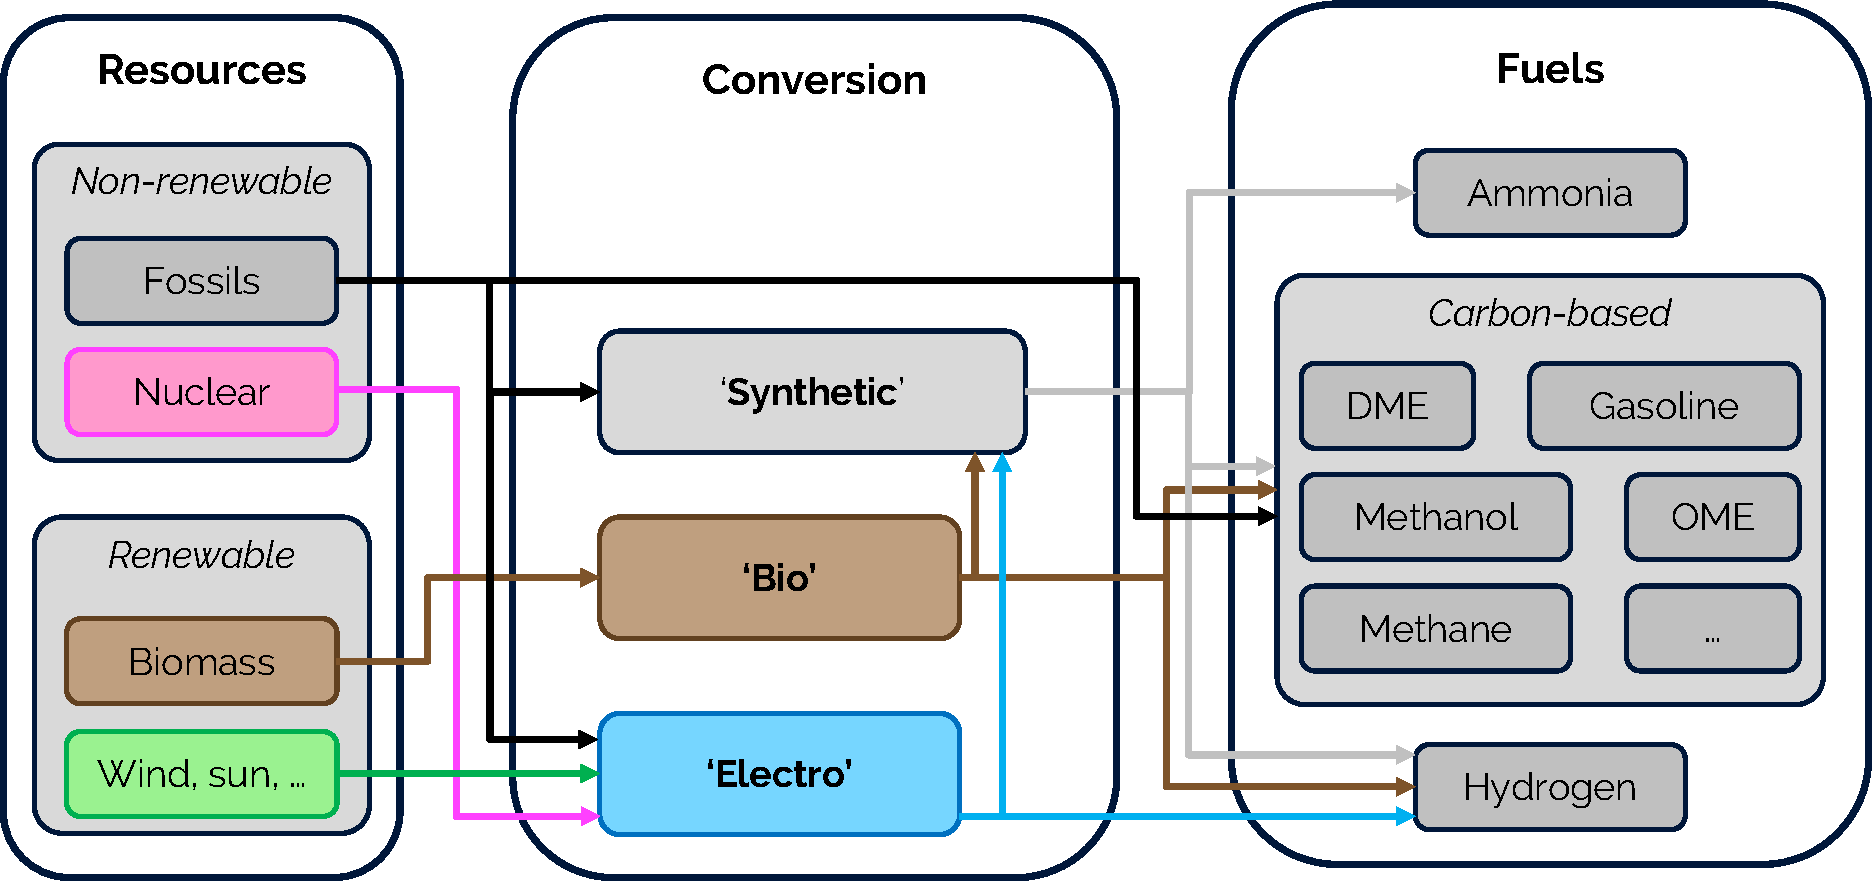
\includegraphics[width=0.9\textwidth]{taxonomy.pdf}
    \caption{Overview of the main pathways to produce fuels. The boxes in the ``conversion" category illustrates the terminology to use in the different cases: first, a fuel can be defined as \emph{bio} or \emph{electro} if the absolute majority of the energy balance of its production consists of biomass or electricity, respectively. Then, a fuel can be defined as \emph{synthetic} if it has been obtained through a synthesis process from another fuel, regardless of the feedstock. The box "Fuels" gives some examples to illustrate the terminology used and applied to very common fuels.}
    \label{fig:synfuels_paths}
\end{figure}

% \textit{Fossil} pathways account, nowadays, for most of the fuels. They are mainly refined from fossil hydrocarbons.  Thus, we define ``\textit{fossil} fuels" as: \textit{fuel based on fossil resources.}

\textit{Biofuels} are those based on biomass as their chemical building blocks and energy supply for their own conversion process (\Cref{fig:synfuels_paths}). Biomass is mainly harvested in a solid form and has a lower energy density than fossil hydrocarbons. Thus, the ``bio" processes aim at concentrating the energy and converting it into a fuel more convenient to use (\eg pellet from woody wastes). %liquid or gaseous fuels.
Similarly to the \citet{OEERE_biofuel}, in the literature, biofuels mainly target liquid or gaseous transport fuels (\eg biodiesel and bioethanol) and imply a sustainable production \cite{eu_biofuel, pottering2009directive}. The definition given by official institutions (\eg the FAO or the European Commission) is aligned with the ISO 16559:2014: ``biofuel is a solid, liquid or gaseous fuel produced directly or indirectly from biomass" \cite{eu_biofuels, FAO_biofuel, ISO16559}. To add a quantitative and measurable aspect in the terminology, we propose the following definition: \textit{biofuels are fuels produced from biomass as the major component of their energy balance}. Even if our terminology lacks the subtlety brought by terms like ``woodfuels", ``agrofuels", or ``municipal by-products", that allow to highlight the source of biomass at stake, provided by the FAO \cite{FAO_biofuel}, this terminology aims at harmonising and desambiguating the meaning of the general term ``biofuel".


%According to the European Commission, biofuels are ``liquid or gaseous transport fuels such as biodiesel and bioethanol which are made from biomass. For biofuels to reduce greenhouse gas emissions without adversely affecting the environment or social sustainability, they must be produced in a sustainable way" \cite{eu_biofuel}. This is also stated in the directive of the European Parliament: ``(10) Biofuel production should be sustainable" \cite{pottering2009directive}. However, this definition is too restrictive as it does not include solid biofuels (\eg bio-char that could replace coke in steel production \cite{mousa2016biomass}) nor biofuels used for other purposes than transport (\ie heat and power). 
%Definition of biomass : ``\textit{the biodegradable fraction of products, waste and residues from agriculture (including vegetal and animal substances), forestry and related industries, as well as the biodegradable fraction of industrial and municipal waste}'' \cite{eu2001directive}. 
 
%For example, the pyrolysis, amongst others, produces coal-chars which is an illustration of a higher energy density fuel produced based on thermo-chemical conversion, or biomethanation which transforms solid digestable biomass into biogas.


\textit{Electrofuels} are, according to \citet{JRC_alternative}, fuels whose energy content comes from renewable electricity. On top of that, \citet{goldmann2018} even add that they should be carbon-neutral and serve as a storage capacity of electricity. To be more comprehensive, we define \textit{electrofuels as fuels produced from electricity}, as the resource used to produce this electricity may vary. This electricity is transformed into hydrogen through electrolysis. This hydrogen can be upgraded in more complex fuels when combined with other molecules (\eg carbon mono/dioxide or nitrogen). Electrofuels group all the fuels where the absolute majority of the energy contained into the fuel comes from electricity. In this sense, it is important to point out that ``electrofuels" do not especially imply ``renewable fuels" (\Cref{fig:synfuels_paths}). For instance, the electricity needed to produce \ce{H2} through an electrolyser can be generated from renewable or non-renewable sources \cite{bhandari2014}, even if the most sustainable way to produce electrofuels remains through the electricity produced in excess from \gls{VRES}.

\textit{Synthetic fuels are fuels which have been obtained through a synthesis process from another fuel}. It encompasses upgrading processes, such as methane produced through the Sabatier process or longer hydrocarbons based on syngas through the Fischer-Tropsch process. We extend the definition of the European Commission and Energy Information Agency who consider synthetic fuels as ``any liquid fuel obtained from coal, natural gas or biomass" \cite{eia2006, eu_synthetic}. By extending this definition and focusing on the synthesis operation, similarly to \citet{speight2020synthetic}, we are able to include emerging fuels like ammonia from the Haber-Bosch process. Contrary to biofuels and electrofuels, the resources used for producing synthetic fuels are not strictly identified. For instance, electrolysis-produced \ce{H2} can be upgraded with synthesis gas from the gasification of biomass to form methanol \cite{mignard2008}. Another example could be the production of ammonia via the synthesis of \ce{H2} from methane-reforming. Consequently, defining a fuel only as ``synthetic" gives a reduced insight about the fuel, especially about its ``renewability". Therefore, we recommend to avoid using ``synthetic fuel". In the former example, one would then rather define the produced methanol as a ``bio-electrofuel" given that its main sources are electricity and biomass. 
% To summarise, we define \textit{synthetic as a generic, and therefore less specific, term that gathers all the aforementioned ones (\ie fossil, bio or electro). Therefore, we recommend to use ``synthetic'' for fuels produced from another one and only when the origin of the resources is not directly identifiable.}
%These fuels cannot be included in the other groups as the used fuel may be produced from different pathways. 
%To summarise, we define synthetic fuel as \textit{a fuel produced from another one; and for which fossil, bio or electro cannot be used.}
%To summarise, we define synthetic fuels as \textit{a fuel produced from another one, where the energy origin used for the fuel cannot be clearly specified. This term is necessary as a synthetic fuel can be produced from a same process but with different resources.}

Finally, besides these recommended terms in the context of the energy transition, others are mainly misleading: ``alternative" or ``non-conventional" fuels. These terms are defined in opposition to another kind of fuels, mostly fossil. However, alternatives of today will be conventions of tomorrow. This means that depending on the ``conventional" of the context, these terms will represent different fuels. Because of this implied ambiguity, we recommend not to use these words as their interpretation is case and time sensitive.

\section{Discussion}
\label{sec:discussion}
% Representing a simple picture with well discerned paths is challenging, as most of the processes can be hybridised, such as gasification with renewable hydrogen injection \textbf{Source}, or electrolysis which can either use fossil or renewable electricity.
In the urging necessity for an energy transition and the persisting need for fuels, technologies to convert primary resources into end-use fuels are rapidly multiplying. In this context, we suggest comprehensive terminology and classification to characterise the fuels. Given the limited insight provided by the widely-used term ``synthetic fuels", we recommend to use more specific terms like ``biofuels", ``electrofuels", or even hybridised terms (\eg ``bio-electrofuels"). These allow to highlight the contribution of biomass and electricity in the energy balance of the fuel.

Giving an exact share of biomass (or electricity) above which a fuel can be defined as biofuel (or electrofuel) would open an endless debate. Therefore, to emphasise the effort to step away from fossil fuels, we suggest to specify the contribution of biomass (or electricity) within the energy balance of the production of the fuel looking at both the feedstock and the energy to supply the conversion or production process. This would give, for instance, ``bio(25) methanol" if 25\% of the energy balance to produce the methanol comes from biomass (\eg biomass gasification). Another example could be ``electro(40) ammonia" if 40\% of the energy balance comes from electricity (\eg water electrolysis, air-captured nitrogen and power supply of the Haber-Bosch process). As electricity can be produced from a wide variety of sources (\Cref{fig:synfuels_paths}), we recommend to give insights on the composition of this electricity (\eg from wind, solar or the grid mix). 

To fully embrace these new terminology and classification, industries and academics will have to switch of perspective as studies on energy balance of biofuels or electrofuels too often consider the energy distribution over the different production steps or the feedstock only rather than over all the resources at stake \cite{OConnell2019,slade2013micro}.



% terms like ``renewable fuels", ``electrofuels", ``biofuels" or ``synthetic fuels" are more and more popular in the literature and used for a vast variety of fuels. These terms imply specific use of primary resources or process. Therefore, they shall be used accurately in order to drive consistent policies and discussions between academia and industries.

% Through a comprehensive literature review, we first identified the top-used term (\ie ``synthetic fuel"), the emergence of new ones like ``electrofuel" and the wide variety of other terms. Then, on the purpose for setting a comprehensive terminology and classification, we pointed out different categories of fuels.

% First of all, the definition of ``renewable fuels" was clearly reminded as fuels produced from non-fossil sources that are naturally replenished on a human timescale. As we aim at a pathway towards sustainability where fuels will keep playing a significant role, the renewable fuels shall gain more and more shares in the global energy mix. Therefore, we recommend to use ``renewable fuel" when it is not produced from fossil sources. Although, we also point out that ``renewable" does not directly mean ``sustainable" as this term implies many more aspects than ``Affordable and Clean Energy" \cite{eu_sustainable}, especially when we consider biofuels (\eg use of lands, indirect impacts on environment).

% Then, besides this first distinction between renewable and non-renewable, mostly fossil fuels, we identified three terms to describe them: ``biofuels", ``electrofuels" and ``synthetic fuels". On one hand, the first two really focus on the resource and the energy balance to produce the fuel. Fuels are defined as ``bio" or ``electro" if a majority of their energy balance (\ie feedstock and energy supply for the conversion processes) consists respectively of biomass or electricity. On the other hand, the last one targets the synthesis process from which a fuel can be produced based on another (or other) one(s). As observed in the literature, this includes many different fuels, from many different processes. Therefore, we encourage to use specific terms like ``biofuels" or ``electrofuels", even hybridised term (\eg ``bio-electrofuels") to give more insight to the reader about the technical implications behind the concerned fuel. 

% Finally, we recommended not to use case and time sensitive terms like ``alternative" or ``non-conventional" fuels, given their ambiguous dependency on the alternatives or conventions which these fuels are opposed to.

% For the purpose of being concise and comprehensive, it is necessary to cluster the fuels in wide aggregates. The objective was to clarify the terminology and propose a classification, mainly based on the used resources. Consequently, there is not a straightforward label corresponding to one fuel. One will have to consider the resources and different process to label the end-use fuel.

% As aforementioned, the innovation is running in the energy sector. Therefore, even if we aim at setting a comprehensive and time insensitive terminology and classification, we do not exclude that, in the coming years, new fuels might emerge and would not fit in our framework.

% As the objective was to clarify the terminology while keeping a simple classification, some processes have been aggregated or not mentioned. As a trade-off between overview and technical insights, technologies were aggregated when their process and inputs were similar, such as thermo-chemical processes, that gather gasification, together with slow or fast pyrolysis. Some technologies are under investigation, such as hydrogen production based on high temperature water cracking from concentrated solar \cite{steinfeld2005solar} or nuclear \cite{fujiwara2008hydrogen} energy.
